\documentclass[a4paper,11pt]{article}
% Various packages
\usepackage{siunitx}
\usepackage[utf8]{inputenc} % æøå
\usepackage[T1]{fontenc} % mere æøå
\usepackage[danish]{babel} % orddeling
\usepackage{verbatim} % så man kan skrive ren tekst
\usepackage{graphicx}
\graphicspath{{assets/}}
\usepackage{a4wide}
\usepackage{url}
\usepackage[left=2cm,top=2cm,bottom=1.5cm,right=2cm]{geometry}
\usepackage{amsmath}
\usepackage{amssymb}
\usepackage{amsthm}
\usepackage{wrapfig}
\usepackage{fixme}
\usepackage{color}
\usepackage[makeroom]{cancel}
\usepackage{pstricks}
\usepackage{pdfpages} % include pdf
\usepackage{forest}
\usepackage{float} % Use [H] in figures
\usepackage{subcaption} % For subfigures
\usepackage{color} % May be necessary if you want to color links
%\usepackage{xcolor} \pagecolor[rgb]{0,0,0} \color[rgb]{1,1,1}
\usepackage{nameref}
\usepackage{hyperref} % Make references clickable
\usepackage[nameinlink,capitalize]{cleveref} % Make eq:refs be in style (1)
\usepackage[linesnumbered, commentsnumbered, lined, ruled, vlined,
%noend  % Have no ⌊-like symbol to indicate end of scope in pseudocode
]{algorithm2e} % Doc: https://goo.gl/6bC1qZ

\crefname{equation}{}{Equations}

% Ændr på navnene der vises når man bruger \autoref{label}
\def\sectionautorefname{Sektion}
\renewcommand{\equationautorefname}{Ligning}
\def\figureautorefname{Figur}
\AtBeginDocument{\renewcommand{\ref}[1]{\autoref{#1}}}

% Sæt \ref{} til at kalde \autoref{}
\AtBeginDocument{\renewcommand{\ref}[1]{\autoref{#1}}}

% Ændr ''*'' i math-felter til \cdot
\DeclareMathSymbol{*}{\mathbin}{symbols}{"01}

% Sæt farver for interne referencer og links
\definecolor{darkblue}{RGB}{25,25,112}
\hypersetup{
	colorlinks=true,    %set true if you want colored links
	linktoc=all,        %set to all if you want both sections and subsections linked
	linkcolor=darkblue, %choose some color if you want links to stand out
	filecolor=blue,     %
	citecolor=black,    %
	urlcolor=cyan,      %
}

% Set indentation to 0:
\setlength\parindent{0pt}

% Keywords relateret til algorithm2e pakken
\newcommand{\True}{\textbf{true}}\newcommand{\False}{\textbf{false}}
\SetStartEndCondition{ }{}{}%
\SetKwProg{Fn}{def}{\string:}{}
\SetKw{KwTo}{to}
\SetKwFor{For}{for}{}{}%
\SetKwFor{ForEach}{foreach}{}{}%
\SetKwIF{If}{ElseIf}{Else}{if}{}{elif}{else}{end}%
\SetKwFor{While}{while}{}{end}\SetKwProg{Fn}{}{}{}
\SetKwInOut{Input}{input}\SetKwInOut{Output}{output}
\setlength{\algomargin}{3em}\DontPrintSemicolon

\newcommand{\longspace}{{\ \ \ \ \ \ \ \ \ \ \ \ \ \ }}
% \renewcommand{\P}{{\mathbb P}}
\newcommand{\R}{{\mathbb R}}
\newcommand{\E}{{\mathbb E}}
\newcommand{\event}{{\mathcal{E}}}
\newcommand{\parfrac}[1]{\frac{\partial}{\partial #1}}
\renewcommand{\num}{{\textrm{num} }}
\newcommand{\size}{{\textrm{size} }}
\newcommand{\ift}{{\textrm{if } }}

\newcommand{\pfrac}[2]{\left( \frac{#1}{#2} \right)}

% Dynamiske (), <>, ceil, floor
\newcommand{\p}[1]{\left( #1 \right)}
\newcommand{\pbig}[1]{\big( #1 \big)}
\newcommand{\pBig}[1]{\Big( #1 \Big)}
\newcommand{\pbigg}[1]{\bigg( #1 \bigg)}
\newcommand{\curly}[1]{\left\{ #1 \right\}}
\renewcommand{\square}[1]{\left[ #1 \right]}
\newcommand{\larr}[1]{\left< #1 \right>}
\newcommand{\ceil}[1]{\left\lceil #1 \right\rceil}
\newcommand{\floor}[1]{\left\lfloor #1 \right\rfloor}

\renewcommand{\P}[1]{\mathbb{P} \square{ #1 } }

\author{Søren Mulvad, rbn601}

\title{Eksamensdisposition - Kapitel 1}

\begin{document}
\maketitle


\begin{itemize}
  \item \textbf{QuickSort}
  \begin{itemize}
    \item Analyse af forventet køretid
  \end{itemize}

  \item \textbf{Min-Cut}
  \begin{itemize}
    \item Håndkørsel
    \item Analyse af sandsynligheden for korrekt svar
  \end{itemize}
\end{itemize}

%%%%%%%%%%%%%%%%%%%%%%%%%%%%%%%%%%%%%%%%%%%%%%%%%%%%%%%%%%%
%%%%%%%%%%%%%%%%%%%%%%%%%%%%%%%%%%%%%%%%%%%%%%%%%%%%%%%%%%%
%%%%%%%%%%%%%%%%%%%%%%%%%%%%%%%%%%%%%%%%%%%%%%%%%%%%%%%%%%%
\newpage
%%%%%%%%%%%%%%%%%%%%%%%%%%%%%%%%%%%%%%%%%%%%%%%%%%%%%%%%%%%
%%%%%%%%%%%%%%%%%%%%%%%%%%%%%%%%%%%%%%%%%%%%%%%%%%%%%%%%%%%
%%%%%%%%%%%%%%%%%%%%%%%%%%%%%%%%%%%%%%%%%%%%%%%%%%%%%%%%%%%
\section{Eksamensdisposition - Kapitel 1}

\subsection{Randomized QuickSort (RQS)}

Vi starter med at definere ''rank'' $i$ af et element, som vi lader være dets position $S_{(i)}$ i det endelige sorterede array (1-indeksering), altså:\\

$S_{(i)}$: Element med rank $i$ (givet 1-indeksering)\\

F.eks.:
\begin{verbatim}
input:  [3, 0, 5, 2] (usorteret array)
output: [0, 2, 3, 5] (sorteret array)
\end{verbatim}
Så vil eksempelvis $S_{(2)} = 2$ og $S_{(4)} = 5$\\


For alle $1 \leq i < j \leq n$ har vi, at $X_{ij} = 1$ hvis $S_{(i)}$ og $S_{(j)}$ sammenlignes af RQS, og 0 ellers. Vi kan gøre det med en simpel indikatorvariabel, da to elementer aldrig kan blive sammenlignet mere end én gang.\\

Da får vi følgende, hvor startgrænsen $j > i$ på det andet sumtegn gælder da sammenligningerne er symmetriske.
$$
  X = \sum_{i=1}^n \sum_{j>i} X_{ij}
$$
\textit{Mål: Find øvre grænse for $\E{X}$}

Nu bruges linearity of expectation:
\begin{align} \label{eq:exp-X}
  \E{X}
  = \E{\sum_{i=1}^n \sum_{j>i} X_{ij}}
  = \sum_{i=1}^n \sum_{j>i} \E{X_{ij}}
  = \sum_{i=1}^n \sum_{j>i} \P{X_{ij} = 1}
\end{align}

Herefter analyserer vi algoritmen:\\
Den fungerer på følgende måde, at hvis vi f.eks. vælger $S_{(4)}$ som pivot i et array med seks elementer vil vi have:
\begin{align} \label{eq:eksempel}
\square{S_{(1)}, S_{(2)}, S_{(3)},} \underbrace{S_{(4)}}_{\text{pivot}}, \square{ S_{(5)}, S_{(6)}}
\end{align}
Herefter vil $S_{(4)}$ aldrig blive sammenlignet med nogle elementer igen, og algoritmen ville nu kigge på de to delarrays der er lavet hver for sig.

Lad os skrive det op mere generelt, hvor vi har to indekser $i,j$ hvor $1 \leq i < j \leq n$. Vi kan da skrive vores array op således:
$$
S_{(1)}, S_{(2)}, S_{(3)}, \cdots, S_{(i)}, \cdots, S_{(j)}, \cdots, S_{(n-1)}, S_{(n)}
$$

Nu vælges en pivot $S_{(k)}$. Da har vi tre mulige cases som beskrevet nedenfor for hvor $k$ vælges:

\begin{enumerate}
	\item $k < i$ eller $k > j$:\\
	$S_{(i)}$ og $S_{(j)}$ bliver ikke sammenlignet i denne iteration af rekursionstræet
	\item $i < k < j$:\\
	$S_{(i)}$ og $S_{(j)}$ sammenlignes \textit{aldrig}. Det skyldes at de vil blive delt ind i hver deres subarray, se evt. \cref{eq:eksempel}.
	\item $k=i$ eller $k=j$:\\
	$S_{(i)}$ og $S_{(j)}$ sammenlignes netop én gang (og herefter aldrig igen).
\end{enumerate}

Vi kan nu i vores analyse ignorere case 1, da $S_{(i)}$ og $S_{(j)}$ ikke sammenlignes her, men vi stadig går et niveau dybere i vores rekursionstræ og der derfor er mulighed for at de sammenlignes senere.\\

Vi ser generelt for case 2 og 3, at de gælder når $i \leq k \leq j$. Case 3 giver os 2 mulige udfald for at de bliver sammenlignet. Antallet af mulige udfald i alt er længden fra $i$ til $j$, som må være $j - i + 1$. Altså får vi:
\begin{align} \label{eq:prob-xij}
  \P{X_{ij} = 1} = \frac{2}{j - i + 1}
\end{align}


Vi benytter nu dette til at regne videre på \cref{eq:exp-X}:
\begin{align}
\E{X} &= \sum_{i=1}^n \sum_{j>i} \P[X_{ij} = 1] \nonumber \\
      &= \sum_{i=1}^n \sum_{j>i} \frac{2}{j - i + 1} \nonumber \\
      &= 2 \sum_{i=1}^n \sum_{j>i} \frac{1}{j - i + 1} \nonumber \\
   &\leq 2 \sum_{i=1}^n \sum_{k=1}^n \frac{1}{k} \label{eq:mindre} \\
      &= 2n \sum_{k=1}^n \frac{1}{k} \nonumber \\
      &= 2n H_n \label{eq:harmonic} \\
      &= O(n \lg n) \nonumber
\end{align}
Ovenfor gælder uligheden ved \cref{eq:mindre}, da $j-i+1 \geq 2$ (da $j$ altid minimum er 1 større end $i$), og $j$ ikke vil gå ''længere ud'' end til $n$.\\
I \cref{eq:harmonic} benytter vi hvad der kaldes det $n$'te Harmoniske tal, som er defineret som $H_n = \sum_{i=1}^n (1/i) = \ln n + \Theta(1)$.\\

Herved kommer vi altså frem til, at $\E{X} = O(n \lg n)$. Da $\E{X}$ er det forventede antal sammenligninger som Randomized QuickSort udfører, må køretiden ligeledes være dette for algoritmen.










\subsection{Forklaring af algoritmen}

Givet en sammenhængende ikke-orienteret graf $G = (V, E)$, da er et min-cut i $G$ en kantmængde $E'$ af minimal størrelse, så $(V, E \backslash E')$ er ikke-sammenhængende.\\

Algoritmen fungerer således:
\begin{itemize}
	\item Vælg kant $e$ uniformt i $E$
	\item Contract $e$ og fjern self-loops
	\item Gentag indtil antal knuder $|V'| = 2$
	\item Returner kantmængde mellem de to knuder
\end{itemize}

\begin{figure}[H]
	\begin{center}
		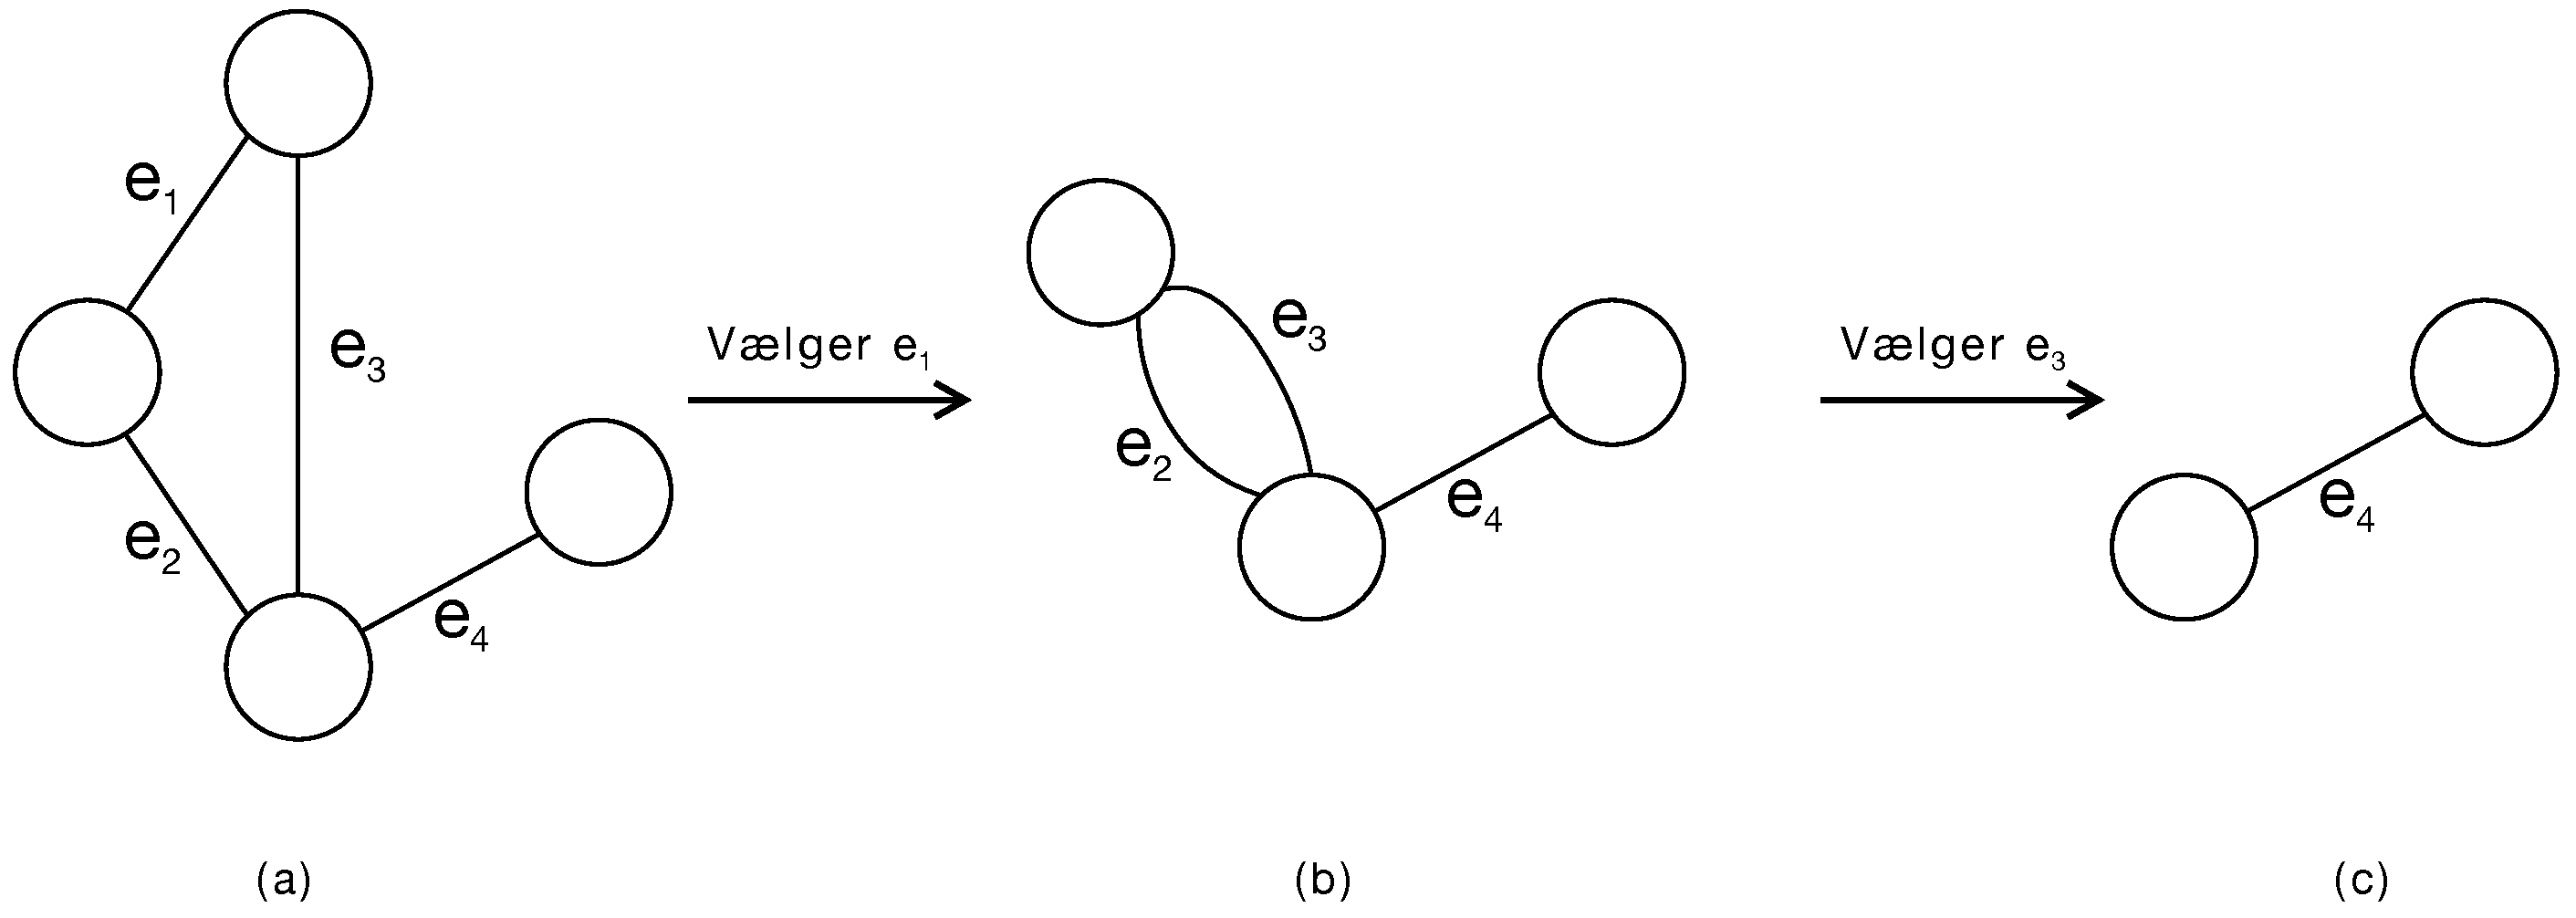
\includegraphics[width=\textwidth]{min-cut.pdf}
	\end{center}
	\caption{Eksempel på Min-Cut}
	\label{fig:min-cut}
\end{figure}

På \ref{fig:min-cut} fra (a) til (b) vælger vi $e_1$. Herved sker der en contraction. Fra (b) til (c) vælger vi $e_3$, hvorved der igen sker en contraction. Vi ser, at vi nu har et self-loop, så det fjerner vi. Nu er der kun to knuder tilbage, så algoritmen er færdig og vi returnerer kantmængden $\{e_4\}$.\\

\textbf{NB:} Bemærk at vi fra (b) til (c) potentielt godt kunne have valgt kant $e_4$, og herved ville vi ikke have fundet et min-cut.





\subsection{Sandsynlighed for succes for én iteration}
Lad os nu betragte et min-cut $C$ og lade $k$ være antallet af kanter i $C$, $k = |C|$. Lad os derudover sige, at $n = |V|$. Og lad os indføre begrebet ''degree'' for hver knude, som beskriver antal kanter der rører knuden.\\

Betragt iteration $i$ hvor $1 \leq i \leq n-2$ (dette er netop det antal iterationer algoritmen vil gå igennem, da vi stopper når der er to knuder tilbage og der fjernes en knude pr. contraction).\\


Antag, at ingen af de kanter der løbende blev contracted i $G$ i iteration $1 \, .. \, i-1$  indgår i vores optimale løsning $C$, således vi ikke potentielt får en fejlagtig løsning.\\

Da der er $n$ knuder til at starte med og der fjernes én pr. contraction, så må der efter $i-1$ iterationer være $n-i+1$ knuder i $G$.\\

Da $k = |C|$ for et min-cut $C$, så må minimum cut-størrelsen i $G$ være $\geq k$. Derfor må der altså også som minimum være $k$ kanter der rører hver knude, så $G_{\text{min\_degree}} \geq k$.\\

Da vi havde, at der var $n-i+1$ knuder i $G$, og vi lige har vist at de alle minimum har degree $k$, så kan vi få et lower bound for antal kanter $|E|$ i $G$:
\begin{align*}
  |E| \geq \frac{(n-i+1)k}{2}
\end{align*}

Her dividerer vi med 2, da vi tager højde for at enhver kant $e$ vil røre to knuder.\\

Således kan vi bestemme sandsynligheden for at en af kanterne i $C$ contractes i iteration $i$ til:
\begin{align} \label{eq:prob-c}
  \P{\text{En kant i $C$ contractes i iteration $i$}} = \frac{k}{|E|} \leq \frac{k}{\frac{1}{2}(n-i+1)k} = \frac{2}{n-i+1}
\end{align}
Dette gælder, da $k$ er antallet af kanter i $C$ og vi ønsker at finde sandsynligheden for at vi tilfældigt vælger en af disse kanter ud af alle kanter $|E|$.\\

Lad os nu definere eventet $\event_i$, som svarer til ''det omvendte'' af eventet beskrevet i \cref{eq:prob-c}\\
$\event_i$: Ingen kant indeholdt i $C$ vælges i iteration $i$.\\

Sandsynlighed for $\event_i$ givet succes i alle foregående iterationer kan herved beskrives som:
\begin{align} \label{eq:prob-succes-given-former-succes}
  \P{ \event_i \middle| \bigcap_{j=1}^{i-1} \event_j} \geq 1 - \frac{2}{n-i+1} = \frac{n-i+1-2}{n-i+1} = \frac{n-i-1}{n-i+1}
\end{align}



\subsection{Sandsynlighed for succes for én hel kørsel}

Da sandsynligheden for at algoritmen terminerer med korrekt resultat svarer til sandsynligheden for at ingen kanter i $C$ vælges i \emph{nogle som helst} af iterationerne (hvor vi tager højde for at der muligvis kan findes flere gyldige min-cut), kan vi benytte \cref{eq:prob-succes-given-former-succes} til at opskrive følgende:
\begin{align}
  \P{\text{Succes}} &\geq \P{ \bigcup_{i=1}^{n-2}   \event_i} \label{eq:p-succes} \\
  &= \P{\event_1} * \P{\event_2 | \event_1} * \P{\event_3 | \event_1 \cap \event_2} \cdots \P{ \event_{n-2} \middle| \bigcap_{i=1}^{n-3} \event_i } \nonumber \\
  &= \prod_{i=1}^{n-2} \P{ \event_i \middle| \bigcap_{j=1}^{i-1} \event_j } \nonumber \\
  &\geq \prod_{i=1}^{n-2} \p{ \frac{n-i-1}{n-i+1} } \label{eq:indsaat-res} \\
  &= \frac{\cancel{(n-2) \cdots 4*3}*2*1 }{n(n-1)\cancel{(n-2) \cdots 4*3} } \nonumber \\
  &= \frac{2}{n(n-1)} \nonumber \\
  &\geq \frac{2}{n^2} \nonumber
\end{align}

I \cref{eq:p-succes} gælder ulighedstegnet, da der muligvis findes flere gyldige min-cuts.\\
I \cref{eq:indsaat-res} indsætter vi vores resultat fra \cref{eq:prob-succes-given-former-succes}.



\subsection{Sandsynlighed for succes givet flere kørsler af algoritmen}
Vi har netop set for den randomiserede min-cut algoritme, at for én kørsel på et input med $n = |V|$, antal knuder, har vi:
$$
  \P{\text{Succes}} \geq \frac{2}{n^2} \quad \Longleftrightarrow \quad \P{\text{Fejl}} \leq 1 - \frac{2}{n^2}
$$

Derudover ved vi, at følgende ulighed gælder for alle $x \in \R$:
\begin{align} \label{eq:exp-regel}
  1 + x \leq e^x
\end{align}

Lad os nu forestille os, at vi kører Min-Cut $k$ gange og returnerer det mindste cut fundet. Denne fremgangsmåde kan kun fejle hvis ingen af kørslerne finder et min-cut. Lad os for at gøre vores analyse nemmere sige vi udfører $k = n^2/2$ kørsler.

\begin{align}
  \P{\text{Fejl med $k$ kørsler}}
  &\leq \p{ 1 - \frac{2}{n^2} }^k \label{eq:koerer-flere-gange} \\
  &\leq \p{e^{- \frac{2}{n^2}}}^k \label{eq:bruger-exp-regel} \\
  &= e^{- \frac{2k}{n^2}} \label{eq:ganger-k-ind} \\
  &= e^{-1} \label{eq:benytter-vaardi-for-k} \\
  &\Updownarrow \nonumber \\
  \P{\text{Succes med $k$ kørsler}} &\geq 1 - e^{-1} \nonumber
\end{align}

I \cref{eq:koerer-flere-gange} ganger vi blot sandsynlighederne for at få fejl $k$ gange sammen.\\
I \cref{eq:bruger-exp-regel} benytter vi reglen i \cref{eq:exp-regel}, hvor $x = -2/n^2$.\\
I \cref{eq:ganger-k-ind} bruger vi potensregler til at sætte $k$ ind i samme potens.\\
I \cref{eq:benytter-vaardi-for-k} benytter vi, at vi sagde vi udførte $k = n^2/2$ kørsler.



\end{document}
